\question \textbf{Maximum likelihood }

The maximum likelihood is a method to find the most suitable phylogenetic tree for a given MSA. Assume that all necessary probabilities are pre-calculated. \\

\begin{figure}[H]
      \centering
      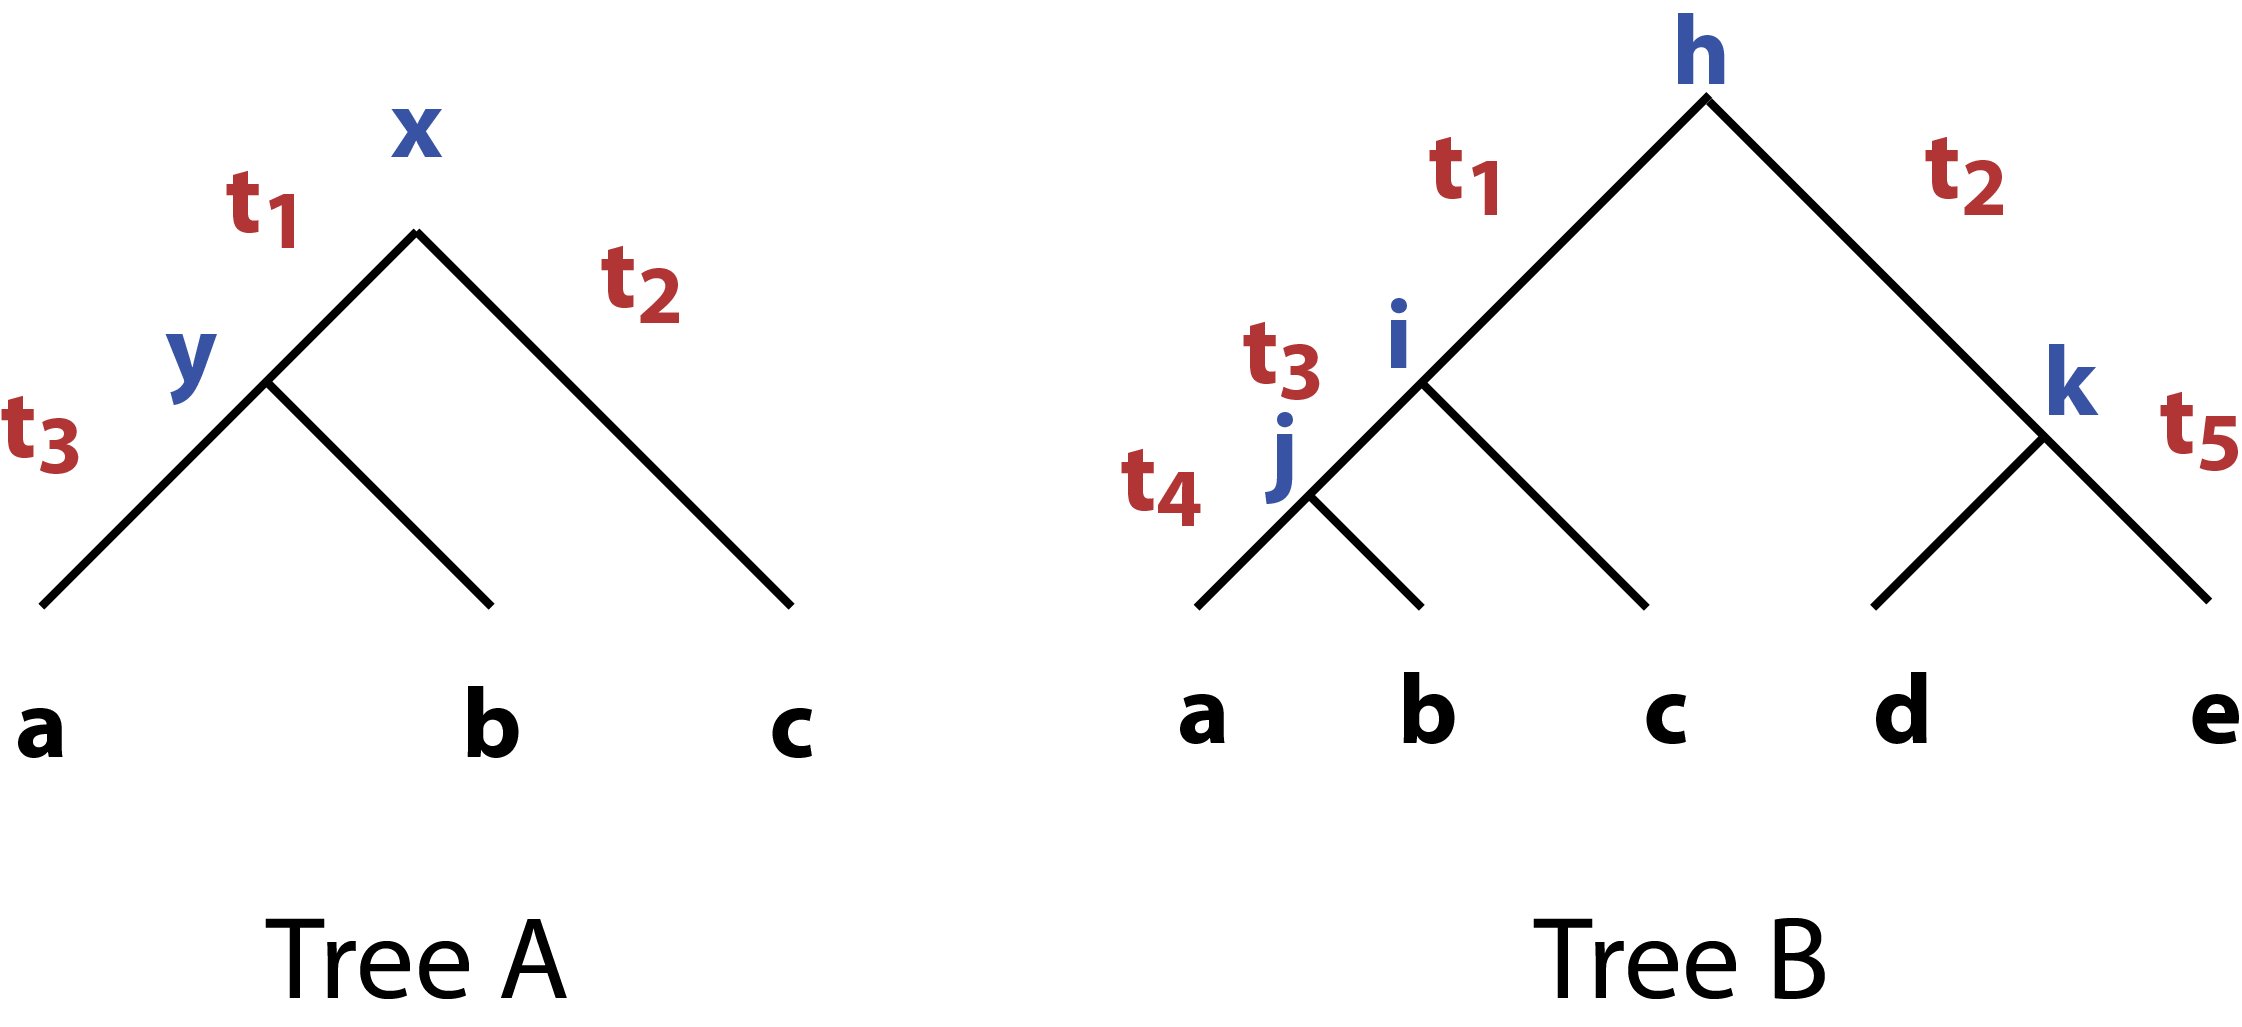
\includegraphics[width=0.5 \textwidth]{fig09/maximum_likelihood.png}
\end{figure}

Use the first column of the MSA and also Tree A and B to answer the following questions.

Likelihood of Tree A: $L(H=Tree A│D=MSA) = p_{xy}(t1)p_{ya}(t3)p_{yb}(t3)p_{xc}(t2)$

\vspace{0.1 in}

\begin{parts}

%% (a)
  \part What is the likelihood of Tree B? Use the same format for Tree A above.

  \medskip 

$L(H=Tree B | D=MSA)$

\begin{solution}[0.35 in]
$p_{hi}(t1)p_{hk}(t2)p_{ij}(t3)p_{ja}(t4)p_{ke}(t5)p_{jb}(t4)p_{ic}(t3+t4)p_{kd}(t5)$
\end{solution}

%% (b)
  \part What is the log-likelihood of Tree A? Use base 2 and the following values for the calculation.
  
\begin{itemize}
\item $p_{xy}(t1)=0.25$
\item $p_{ya}(t3)= 0.0625$
\item $p_{yb}(t3)=0.0625$
\item $p_{xc}(t2)= 0.125$
\end{itemize}

\medskip 

\begin{itemize}
\item $2^(-2)=0.25$
\item $2^(-3)=0.125$
\item $2^(-4)=0.0625$
\end{itemize}

\medskip
  
$L(H=Tree A | D=MSA)$

\begin{solution}[1.75 in]
\quad \linebreak 
$\log_{2}⁡p_{xy}(t1) + \log_{2⁡}p_{ya}(t3) + \log_{2⁡}p_{yb}(t3) + \log_{2⁡}p_{xc}(t2)$ \\
$=\log_{2⁡}0.25 +\log_{2⁡}0.0625 + \log_{2}⁡0.0625 + \log_{2⁡}0.125$ \\
$= -2-4-4-3$ \\
$=-13$
\end{solution}

\end{parts}

